\documentclass[
	a4paper, % Paper size, use either a4paper or letterpaper
	12pt, % Default font size, the template is designed to look good at 12pt so it's best not to change this
	%unnumberedsections, % Uncomment for no section numbering
]{article}
\usepackage[a4paper,top=0.4cm, bottom=1.6cm, left=1.6cm, right=1.6cm]{geometry}

\usepackage{cmap} % make PDF files searchable and copy-able
\usepackage[utf8]{inputenc}
\usepackage[english,russian]{babel}

\usepackage{amssymb,amsmath}
\renewcommand {\phi}{\varphi}
\usepackage{mathtext}

\usepackage{libertine}
\usepackage[libertine]{newtxmath}

\usepackage{graphicx} % Required for inserting images
\graphicspath{{./img/}} % Destination of images
\usepackage{subcaption}

\usepackage{hyperref}



% opening
\title{Отчет о выполнении лабораторной работы 1.2.1\\Определение скорости полета пули при помощи баллистического маятника}
\author{Шубин Владислав}
\date{Сентябрь 2023}

\begin{document}    
	
	\maketitle
	
	\section{Аннотация}
	В работе определяется скорость полета пули, путём применения законов сохранения и использования баллистического маятника. Используется следующий метод измерений скорости: 1) определение отклонения маятника с помощью оптической системы, изображенной на рис. \ref{fig:subim1} Геометрические размеры образца измеряются с помощью линейки, штангенциркуля и микрометра. Детально исследуется систематические и случайные погрешности проводимых измерений.
	
	
	\section{Теоретические сведения}
	
	\subsection{Метод баллистического маятника, совершающего поступательное движение}
	
	В этой части работы (вторая часть не выполнялась) используется установка, изображенная на рис. \ref{fig:subim1}. Внешними силами для системы пуля-цилиндр являются сила тяжести, не имеющая горизонтальной компоненты, и силы натяжения нитей, горизонтальные компоненты которых появляются при отклонении маятника. Но так как отклонения маятника малы, то и эти компоненты малы и тем более мал и их импульс. Поэтому закон сохранения импульса при соударении пули с цилиндром имеет вид
	\begin{equation}
		mu = (M + m)V.
	\end{equation}
	Здесь m - масса пули, M - масса цилиндра, V - скорость цилиндра и пули после неупругого соударения.
	
	Откуда (учитывая, что M >> m) можно написать
	\begin{equation}
		u = \frac{M}{m}V.
	\end{equation}
	
	По закону сохранения энергии
	
	\begin{equation}
		V^2 = 2gh.
	\end{equation}
	Здесь g - ускорение свободного падения, h - высота подъёма маятника над его начальным положением.
	
	Высота подъёма маятника выражается через угол $\phi$ отклонения маятника от вертикали:
	\begin{equation}
		h = L(1 - \cos{\phi}) = 2L\sin^2{\frac{\phi}{2}},
	\end{equation}
	где $\phi$ $\approx$ $\frac{\Delta x}{L}$
	
	Из (2), (3) и (4) получаем формулу для определения скорости пули:
	\begin{equation}
		v = \frac{M}{m}\sqrt{\frac{g}{L}}\Delta x.
	\end{equation}
	
	
	\begin{figure}[h]
		
		\begin{subfigure}{0.5\textwidth}
			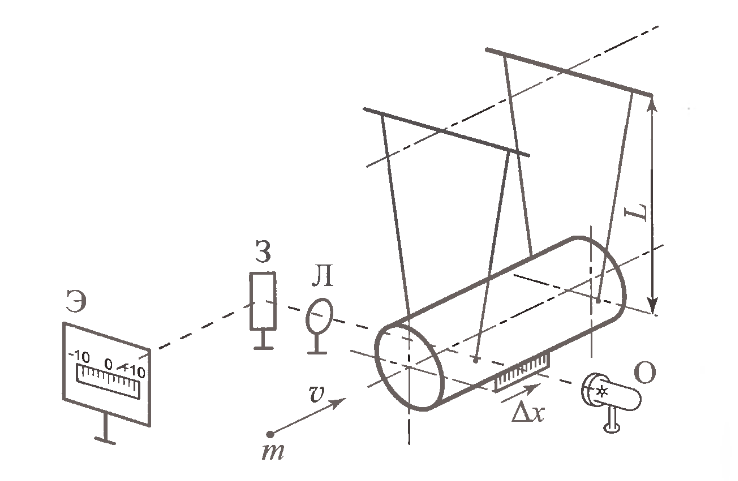
\includegraphics[width=0.9\linewidth]{1.png} 
			\caption{Рис. 1. Схема установки для измерения скорости полета пули}
			\label{fig:subim1}
		\end{subfigure}
		\begin{subfigure}{0.5\textwidth}
			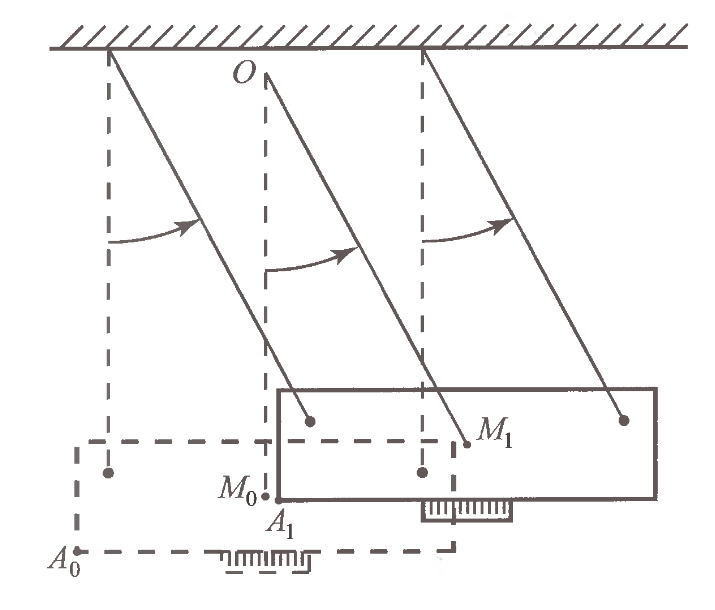
\includegraphics[width=0.9\linewidth]{2.png}
			\caption{Рис 2. Поведение баллистического маятника при попадании в него пули}
			\label{fig:subim2}
		\end{subfigure}
		
	\end{figure}
	
	\section{Оборудование и инструментальные погрешности}
	\textbf{Оборудование:} духовое ружье на штативе, осветитель, оптическая система для измерения отклонений маятника, измерительная линейка, пули и весы для их взвешивания, а также баллистические маятники.
	\begin{itemize}
		\item Линейка: $\Delta \text{лин}$ = $\pm$0.5 мм (по цене деления).
		\item Весы: $\Delta m = 0.001\text{ г}$
	\end{itemize}
	
	\section{Результаты измерений и обработка данных}
	\subsection{Массы пулек:}
	
	\begin{figure}[h]
		\begin{center}$
			\begin{array}{|c|c|c|c|c|c|c|c|c|c|c|}
				\hline
				N \text{изм.} & 1 & 2 & 3 & 4 & 5 & 6 & 7 & 8 & 9 & 10  \\
				\hline
				m\text{, г} & 0.516 & 0.515 & 0.503 & 0.504 & 0.507 & 0.512 & 0.508 & 0.507 & 0.509 & 0.501 \\
				\hline
			\end{array}$
		\end{center}
	\end{figure}
	
	$L = (2220\pm10)$ мм, $M=(2900\pm5)$ г.
	
	\subsection{Амплитуды и соответствующие скорости:}
	
	\begin{figure}[h]
		\begin{center}$
			\begin{array}{|c|c|}
				\hline
				\Delta x\text{, мм} & v\text{, м/c} \\
				\hline
				11.7\pm0.2 & 135.24\pm3 \\
				\hline
				10.2\pm0.2 & 140.57\pm3 \\
				\hline
				11.7\pm0.2 & 146\pm3 \\
				\hline
			\end{array}$
		\end{center}
	\end{figure}
	
	Усредняя, получаем $v=(140\pm5)\text{, м/c}$.
	\section{Обсуждение результатов}
	
	\section{Заключение}
	Я получил значение скорости пули методом баллистического маятника. Значения скорости совпали с точностью до погрешности, в том числе и с остальными студентами моей группы.
	
	
\end{document}
